\section{Математическое описание}

\subsection{Граф и его определение}

Граф~-- пара $G = (V, E)$, где $V$~-- конечное непустое множество вершин,
$E \subseteq V \times V$~-- множество рёбер. Граф называется ориентированным,
если каждое ребро~-- упорядоченная пара, и неориентированным в противном
случае. Ациклический граф не содержит циклов; связный ациклический
неориентированный граф является деревом, ориентированный~-- DAG
(directed acyclic graph).

Взвешенный граф задаёт функцию весов $w : E \to \mathbb{R}$, ставящую
каждому ребру вещественное число. В данной работе веса генерируются
по распределению Вейбулла.

\subsection{Распределение классического Вейбулла}
Для генерации случайных значений используется форума из учебника \cite{vadzinsky}
\[
X = a\,(-\ln r)^{1/c}, \text{где } r \in (0, 1)
\]
Это позволяет получить значения, распределённые по закону Вейбулла, что
делает генерацию параметров графа более реалистичной и менее равномерной
по сравнению с обычным генератором случайных чисел.

В реализации используются два независимых экземпляра распределения
с параметрами \texttt{a = 10, c = 2}: один для генерации структуры графа
(степеней вершин), другой~-- для генерации весов рёбер.

На рисунке \ref{fig:weibull} показана график распределения из учебника.
\begin{figure}[H]
    \centering
    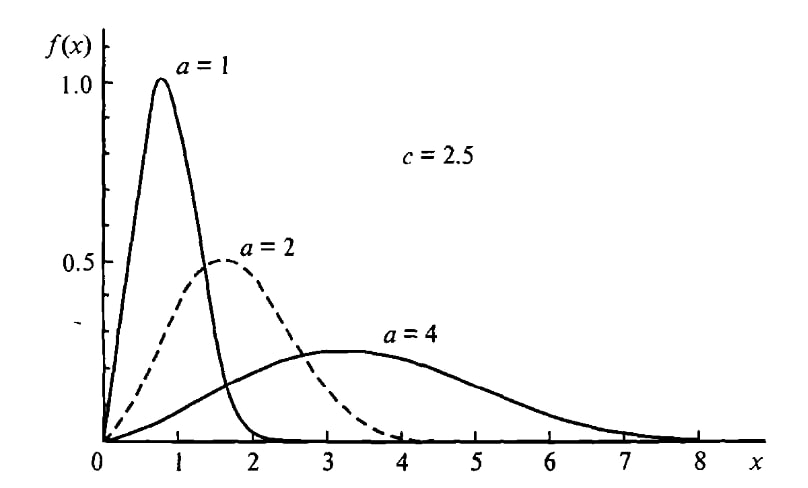
\includegraphics[width=0.8\textwidth]{photo/wei.jpg}
    \caption{Распределение Вейбулла}
    \label{fig:weibull}
\end{figure}

На рисунке~\ref{fig:weibull_my} показана гистограмма 1000 сгенерированных
значений и теоретическая плотность распределения.

\begin{figure}[H]
    \centering
    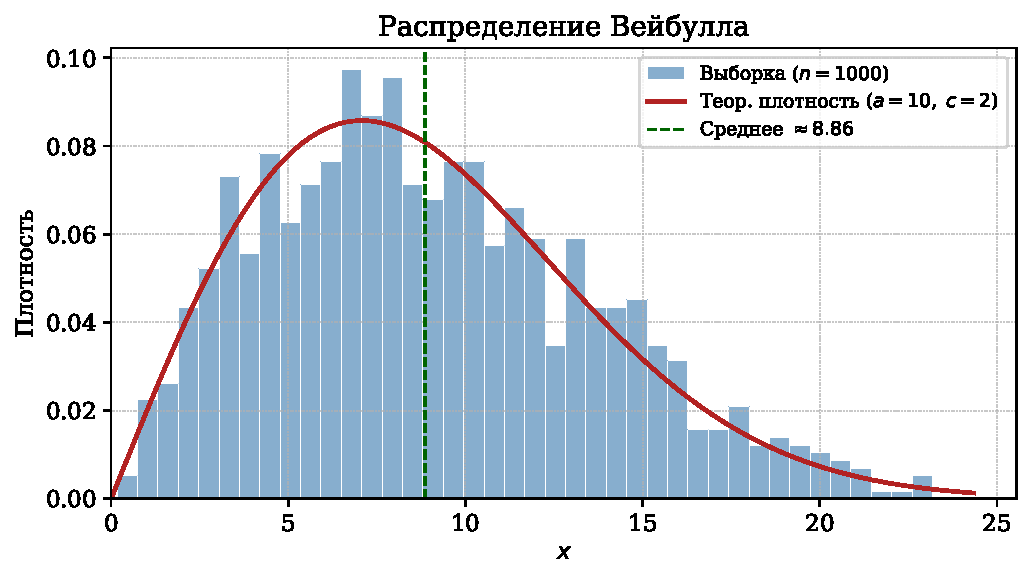
\includegraphics[width=0.8\textwidth]{photo/weibull_plot.pdf}
    \caption{Распределение Вейбулла ($a=10,\; c=2$): выборка $n=1000$
             и теоретическая плотность}
    \label{fig:weibull_my}
\end{figure}

\subsection{Генерация связного ациклического графа по степеням вершин}

Пользователь задаёт число вершин $n$, тип ориентированности и знак весов.
Число рёбер не вводится напрямую.

\textbf{Шаг~1: генерация целевых степеней.}
Для каждой вершины $i \in \{0,\ldots,n-1\}$ генерируется
значение по распределению Вейбулла, округляемое до целого числа
в диапазоне $[1,\,\lfloor\log n\rfloor]$:
\[
    d_i = \max\!\bigl(1,\;\min\!\bigl(\lfloor X_i \rfloor,\;
    \lfloor\log n\rfloor\bigr)\bigr),
    \quad X_i \sim \mathrm{Weibull}(a,\,c).
\]

\textbf{Шаг~2: формирование остовного дерева.}
Для каждой вершины $\pi[i]$ при $i \geq 1$ случайный предок выбирается
равновероятно из $\{\pi[0],\ldots,\pi[i-1]\}$ и добавляется направленное
ребро $\pi[j] \to \pi[i]$.
Поскольку $j < i$ для всех добавляемых рёбер, ни одно ребро не идёт
«назад» в топологическом порядке, что гарантирует ациклическость.
После этого шага граф связен и содержит ровно $n-1$ рёбер.

\textbf{Шаг~3: добирание дополнительных рёбер.}
Для каждой вершины $\pi[i]$ формируется множество допустимых целей:
\[
    T_i = \bigl\{\,j \;\big|\; j > i,\;
    (\pi[i],\,\pi[j]) \notin E\,\bigr\}.
\]
Множество $T_i$ случайно перемешивается, где индексы
генерируются по распределению Вейбулла.
Затем добавляются первые
$\min\!\bigl(d_i,\,|T_i|\bigr)$ рёбер из перемешанного списка.
Условие $j > i$ сохраняет инвариант ациклическости:
все рёбра по-прежнему направлены в сторону возрастания индекса.

\textbf{Учёт ориентированности и весов.}
Для неориентированного графа каждое ребро $u \to v$ добавляется симметрично:
дополнительно добавляется $v \to u$ с тем же весом.
Вес каждого ребра генерируется из и распределения Вейбулла
и при необходимости меняет знак согласно выбранному режиму
(\texttt{POSITIVE}, \texttt{NEGATIVE}, \texttt{MIXED}).

\subsection{Эксцентриситет, центр и диаметральные вершины}

\textit{Эксцентриситетом} $e(v)$ вершины $v$ в связном графе $G(V, E)$
называется максимальное расстояние от вершины $v$ до других вершин графа $G$:
\[
e(v) \stackrel{\text{Def}}{=} \max_{u \in V} d(v, u).
\]

\textit{Радиусом} $R(G)$ графа $G$ называется наименьший из эксцентриситетов вершин:
\[
R(G) \stackrel{\text{Def}}{=} \min_{v \in V} e(v).
\]

Вершина $v$ называется \textit{центральной}, если её эксцентриситет совпадает
с радиусом графа, $e(v) = R(G)$. Множество центральных вершин называется
\textit{центром} графа:
\[
C(G) \stackrel{\text{Def}}{=} \{v \in V \mid e(v) = R(G)\}.
\]

Диаметральные вершины~-- с максимальным эксцентриситетом:
\[
D(G) = \{v \mid e(v) = \mathrm{diam}(G)\}.
\]

Расстояния вычисляются алгоритмом обхода в ширину ($BFS$), запускаемым
из каждой вершины; алгоритмическая сложность линейная ($O(V + E)$) для
одного прохода, а итоговая сложность квадратична $O(V(V + E))$.

\subsection{Метод Шимбелла}

\begin{enumerate}
    \item Операция умножения двух величин $a$ и $b$ при возведении матрицы
    в степень соответствует их алгебраической сумме:
    \begin{equation}
        a \cdot b = b \cdot a \Rightarrow a + b = b + a, \qquad
        a \cdot 0 = 0 \cdot a = 0 \Rightarrow a + 0 = 0.
    \end{equation}

    \item Операция сложения двух величин $a$ и $b$ заменяется выбором
    минимального (максимального) элемента из ненулевых:
    \begin{equation}
        a + b = b + a = \min(\max)\{a, b\}.
    \end{equation}
    Нули при этом игнорируются: минимальный или максимальный элемент
    выбирается из ненулевых значений. Нуль в результате операции может быть
    получен лишь тогда, когда все слагаемые -- нулевые.
\end{enumerate}

Элемент матрицы $A^{(2)}$, полученной возведением $A$ в степень~2,
вычисляется как:
\[
\omega_{ij}^{(2)} = \min(\max) \left\{
    \omega_{i1}^{(1)} + \omega_{1j}^{(1)},\;
    \omega_{i2}^{(1)} + \omega_{2j}^{(1)},\;
    \ldots,\;
    \omega_{in}^{(1)} + \omega_{nj}^{(1)}
\right\}.
\]
Матрица $A^{(k)}$, вычисленная последовательным умножением, содержит длины
путей из ровно $k$ рёбер для всех пар вершин. Временная сложность: $O(k \cdot n^3)$,
пространственная: $O(n^2)$.

\subsection{Упорядочивание графа по алгоритму Фалкерсона}

Алгоритм Фалкерсона -- графический метод топологической сортировки DAG,
состоящий из следующих шагов.

\begin{enumerate}
    \item Найти вершины графа, в которые не входит ни одна дуга.
    Они образуют первую группу. Пронумеровать вершины группы в произвольном порядке.

    \item Вычеркнуть все пронумерованные вершины и дуги, из них исходящие.
    В получившемся графе найдётся, по крайней мере, одна вершина, в которую
    не входит ни одна дуга. Этой вершине, входящей во вторую группу, присвоить
    очередной номер и так далее. Второй шаг повторять до тех пор, пока не будут
    упорядочены все вершины.
\end{enumerate}

Если на каком-либо шаге вершин без входящих дуг не оказалось, граф содержит
цикл и алгоритм неприменим. Алгоритмическая сложность: $O(V^2)$ в матричном
представлении, поскольку на каждом шаге выполняется просмотр всей матрицы
смежности для поиска вершин без входящих дуг.

\subsection{Нахождение кратчайшего пути. Алгоритм Флойда-Уоршалла}

Алгоритм Флойда-Уоршалла находит кратчайшие пути между \textit{всеми} парами
вершин в ориентированном взвешенном графе.

Для хранения информации о путях используется матрица $H$ размера $n \times n$:
\[
H[i, j] =
\begin{cases}
    k, & \text{если $k$~-- первая вершина, достигаемая на кратчайшем
    пути из $i$ в $j$;} \\
    -1, & \text{если из вершины $i$ в вершину $j$ нет пути.}
\end{cases}
\]

Основной цикл: для каждой промежуточной вершины $k$ проверяется
\[
    \text{если } d[i][k] + d[k][j] < d[i][j], \quad
    \text{то } d[i][j] \leftarrow d[i][k] + d[k][j], \quad H[i][j] \leftarrow H[i][k].
\]

\textbf{\textit{Если в $G$ есть цикл с отрицательным весом, то решения
поставленной задачи не существует.}}

Алгоритмическая сложность: $O(n^3)$, пространственная: $O(n^2)$.

\subsection{Определение сети}

Пусть $G = (V, E)$ — орграф с одним источником $s \in V$ и
одним стоком $t \in V$, где $s \neq t$.

\textbf{Сетью} $S = (G;\, c)$ назовём орграф $G$ с заданной функцией
$c : E \to \mathbb{R}_+$, сопоставляющей каждой дуге $e \in E$
неотрицательное действительное число $c(e)$, называемое
\textit{пропускной способностью} этой дуги.

\subsection{Поток в сети}

\textbf{Потоком} в сети $S = (G;\, c)$, где $G = (V, E)$, называется такая
функция $f : E \to \mathbb{R}_+$, приписывающая каждой дуге $e \in E$
неотрицательное число $f(e)$, называемое \textit{потоком} по этой
дуге $e$, для которой выполняются свойства:

\begin{enumerate}
    \item для каждой дуги $e \in E$ верно $f(e) \leqslant c(e)$,
    т.\,е. поток по любой дуге не превышает пропускной способности этой дуги;

    \item для каждой вершины $v \in V$, $v \neq s,\, t$, верно
    \[
        D_f(v) = \sum_{e \in A(v)} f(e) - \sum_{e \in B(v)} f(e) = 0,
    \]
    т.\,е. поток, входящий в любую вершину, кроме источника и стока,
    без остатка выходит из неё (сохранение потока).
\end{enumerate}

При этом неотрицательное число
\[
    p_f = \sum_{e \in A(s)} f(e)
\]
называется \textbf{величиной потока} $f$.

\subsection{Алгоритм Форда--Фалкерсона}

\textbf{Теорема} (Л.\,Р.\,Форд, Д.\,Р.\,Фалкерсон, 1962).
\textit{Величина максимального потока $p_{\max}$ в сети $S$ совпадает
с минимальной пропускной способностью $r_{\min}$ её разрезов.}

Алгоритм итеративно строит максимальный поток от истока $s$ к стоку $t$.
На каждой итерации через BFS ищется кратчайший увеличивающий путь $P$
в остаточной сети, где пропускная способность остаточного ребра:
\[
    r(u,v) = c(u,v) - f(u,v).
\]
Величина дополнительного потока определяется узким местом пути:
\[
    \Delta f = \min_{(u,v) \in P} r(u,v).
\]
Для каждого ребра $(u,v)$ пути $P$ остаточная сеть обновляется:
\[
    r(u,v) \leftarrow r(u,v) - \Delta f, \quad
    r(v,u) \leftarrow r(v,u) + \Delta f.
\]
Величина потока увеличивается на $\Delta f$:
\[
    f \leftarrow f + \Delta f.
\]
Алгоритм завершается, когда BFS не находит пути от $s$ до $t$.

\subsection{Нахождение заданного потока минимальной стоимости}

Рассмотрим задачу определения потока заданной величины $\theta$ от $s$ к
$t$ в сети $G = (S, U, \Omega, D)$, в которой каждая дуга $(x_i, x_j)$
характеризуется пропускной способностью $c(x_i, x_j) \in \Omega$ и
неотрицательной стоимостью $d(x_i, x_j) \in D$.

Математическая модель задачи: минимизировать
\[
    \sum_{(x_i,\, x_j) \in U} d(x_i, x_j) \cdot \varphi(x_i, x_j),
\]
при ограничениях:

\begin{enumerate}
    \item $0 \leqslant \varphi(x_i, x_j) \leqslant c(x_i, x_j)$
          для всех $(x_i, x_j) \in U$;
    \item для истока $s$:
          $\displaystyle\sum_{x_j} \varphi(s, x_j) - \sum_{x_j} \varphi(x_j, s) = \theta$
    \item для стока $t$:
          $\displaystyle\sum_{x_j} \varphi(t, x_j) - \sum_{x_j} \varphi(x_j, t) = -\theta$
    \item для любой другой вершины: условие сохранения потока равно нулю.
\end{enumerate}

\subsection{Теорема Кирхгофа}

Пусть $G = (V, E)$~-- связный неориентированный граф без петель и кратных
рёбер, $|V| = n$. \textit{Матрица Кирхгофа} $B = D - A(G)$,
где $D = \mathrm{diag}(\deg v_1, \ldots, \deg v_n)$~-- диагональная матрица
степеней вершин, $A(G)$~-- матрица смежности:
\[
    b_{ij} =
    \begin{cases}
        \deg v_i, & i = j, \\
        -1,       & i \neq j,\ v_i \sim v_j, \\
        0,        & i \neq j,\ v_i \not\sim v_j.
    \end{cases}
\]

\textbf{Теорема} (матричная теорема Кирхгофа). Число остовных деревьев в связном
графе G порядка n ≥ 2 равно алгебраическому
дополнению любого элемента матрицы Кирхгофа $B(G)$

\subsection{Алгоритм Краскала}

Алгоритм перебирает рёбра графа в порядке возрастания веса и жадно
добавляет каждое ребро в остов, если оно не создаёт цикл.

Рёбра сортируются по весу: $w(e_1) \leqslant w(e_2) \leqslant \ldots
\leqslant w(e_m)$. Затем для каждого ребра $(u, v)$ проверяется
существование пути между $u$ и $v$ в уже построенной части дерева $T$.
Если путь есть — добавление ребра создало бы цикл, поэтому оно
пропускается. Если пути нет — ребро добавляется в $T$.

Алгоритм завершается когда $|T| = n - 1$, то есть все вершины
связаны минимальным числом рёбер без циклов.
Суммарный вес полученного остова:
\[
    W = \sum_{(u,v) \in T} w(u,v).
\]

\subsection{Код Прюфера}

\textbf{Кодирование (дерево~$\to$~код Прюфера).}
Алгоритм итеративно удаляет листья дерева.
На каждом шаге среди всех вершин находится лист
с минимальным номером.
Сосед этого листа записывается в последовательность кода,
после чего лист удаляется из дерева и степени обновляются.
Процесс повторяется $n-2$ раза.
В результате получается последовательность длины $n-2$:
\[
    \text{код} = (a_1,\, a_2,\, \ldots,\, a_{n-2}),
\]
где каждый элемент $a_i$ -- сосед удалённого на шаге $i$ листа.

\textbf{Декодирование (код Прюфера~$\to$~дерево).}
На каждом шаге среди всех активных вершин ищется минимальная,
которая не встречается в оставшейся части кода~-- она является листом.
Найденный лист соединяется ребром с текущим элементом кода,
после чего лист помечается как удалённый и код сдвигается вперёд.
После обработки всех $n-2$ элементов кода две оставшиеся активные
вершины соединяются последним ребром.
В результате восстанавливается исходное дерево с $n-1$ рёбрами.

\subsection{Максимальное независимое множество вершин}

\textbf{Максимальное независимое множество вершин.}
Множество вершин $S \subseteq V$ называется \textit{независимым},
если никакие две вершины из $S$ не смежны:
\[
    \forall\, u, v \in S \colon (u, v) \notin E.
\]
\textit{Максимальным} независимым множеством называется независимое
множество наибольшей мощности~-- то есть такое $S^*$, что
$|S^*| \geqslant |S|$ для любого другого независимого множества $S$.

\textbf{Алгоритм поиска максимального независимого множества.}
Алгоритм перебирает все возможные подмножества вершин с помощью
рекурсивного возврата.

Начинаем с пустого множества $S$ и полного списка кандидатов $T$,
содержащего все вершины графа.
Для каждой вершины $v$ из списка кандидатов проверяем:
есть ли ребро между $v$ и хотя бы одной вершиной из $S$?
Если ребра нет~-- $v$ можно добавить в $S$ без нарушения независимости.

После добавления $v$ в $S$ формируется новый список кандидатов~--
из $T$ убираются сама вершина $v$ и все её соседи,
так как они уже не могут войти в независимое множество вместе с $v$.
Далее алгоритм рекурсивно продолжает перебор с обновлёнными $S$ и $T$.

Если размер текущего $S$ превышает размер лучшего найденного
множества~-- сохраняем $S$ как новый ответ.

Когда список кандидатов $T$ опустеет~-- ветка заканчивается
и алгоритм возвращается назад, пробуя следующую вершину.
После перебора всех ветвей в $S^*$ будет лежать максимальное
независимое множество.

\subsection{Эйлеровы графы}

Если граф имеет цикл (не обязательно простой), содержащий все рёбра графа, то такой цикл называется \textit{эйлеровым циклом}, а граф называется \textit{эйлеровым графом}.  
Если граф имеет цепь (не обязательно простую), содержащую все рёбра, то такая цепь называется \textit{эйлеровой цепью}, а граф называется \textit{полуэйлеровым графом}.

Эйлеров цикл содержит не только все рёбра (по одному разу), но и все вершины графа (возможно, по несколько раз). Ясно, что эйлеровым может быть только связный граф.


\textbf{Теорема:} Если граф $G$ связан и нетривиален, то следующие утверждения эквивалентны:
\begin{enumerate}
    \item $G$ - эйлеров граф.
    \item Каждая вершина $G$ имеет чётную степень.
    \item Множество рёбер $G$ можно разбить на простые циклы.
\end{enumerate}

\subsection{Достройка до эйлерового графа}

Алгоритм итеративно устраняет вершины нечётной степени.

На каждой итерации собирается список вершин с нечётной степенью.
Если список пуст~-- граф уже эйлеров, алгоритм завершается.

Иначе перебираются все пары нечётных вершин $(u, v)$ и для каждой
пары выполняется одно из трёх действий:

\begin{enumerate}
    \item если ребро $(u, v)$ отсутствует~-- добавляем его.
    Степени обеих вершин увеличиваются на~1 и становятся чётными;

    \item если ребро $(u, v)$ существует и не является мостом~--
    удаляем его. Степени обеих вершин уменьшаются на~1
    и становятся чётными. Мост проверяется через BFS:
    ребро $(u,v)$ удаляется из рабочей копии матрицы смежности,
    после чего проверяется достижимость $v$ из $u$;
    если $v$ недостижима~-- ребро является мостом;

    \item если ребро $(u, v)$ существует и является мостом~--
    пара пропускается, переходим к следующей.
\end{enumerate}

Если за одну итерацию не удалось исправить ни одну пару~--
алгоритм завершается. По завершении граф является эйлеровым
(все степени чётные), полуэйлеровым (ровно две нечётные вершины)
или не эйлеровым (более двух нечётных вершин).

\subsection{Алгоритм построения эйлерова цикла}

\textbf{Алгоритм построения эйлерова цикла.}
Алгоритм строит эйлеров цикл с помощью стека.

В качестве стартовой выбирается любая вершина с ненулевой степенью.
Стартовая вершина помещается в стек $S$.

Пока стек не пуст выполняется следующее.
Смотрим на верхнюю вершину $v$ стека.
Если из $v$ есть хотя бы одно непройденное ребро~--
берём первого доступного соседа $u$, помещаем $u$ в стек
и удаляем ребро $(v, u)$ из рабочей копии матрицы смежности.
Если из $v$ нет непройденных рёбер~--
извлекаем $v$ из стека и добавляем в результат.

После завершения проверяется корректность: если длина результата
не равна числу рёбер плюс один~-- цикл не найден.
В противном случае результат содержит последовательность вершин
эйлерова цикла.

\subsection{Фундаментальная система циклов и циклический ранг}

Пусть $T(V, E_T)$ - некоторый остов графа $G(V, E)$.  
\textit{Кодеревом} $T^*(V, E_T^*)$ остова $T$ называется остовный подграф, такой что $E_T^* = E \setminus E_T$. Рёбра кодерева называются \textit{хордами} остова. Каждая хорда $e \in E_T^*$ остова $T$ порождает ровно один простой цикл, обозначим его $Z_e$.  
Таким образом, имеем систему простых циклов



\[
Z \stackrel{\text{Def}}{=} \{ Z_e \}_{e \in E_T^*},
\]



определяемых выбранным остовом $T$, которая называется \textit{фундаментальной системой циклов}.  
Циклы фундаментальной системы называются \textit{фундаментальными циклами}, а количество циклов в данной фундаментальной системе называется \textit{циклическим рангом} (или \textit{цикломатическим числом}) графа $G$ и обозначается $m(G)$.


\subsection{Симметрическая разность циклов}

Любой цикл в связном графе $G(V, E)$ можно представить как симметрическую разность нескольких фундаментальных циклов из системы $Z$, определяемой произвольным остовом $T$.

\textit{Симметрической разностью} двух множеств рёбер $Z_a$ и $Z_b$ называется
\[
    Z_a \mathbin{\triangle} Z_b
    = (Z_a \setminus Z_b) \cup (Z_b \setminus Z_a),
\]
то есть множество рёбер, принадлежащих ровно одному из двух циклов.